\section{Problem (5)}
	The two vectors $\vec{a}$ and $\vec{b}$ in \cref{fig:hw3_problem5} have equal magnitudes of $42 \ ft$ and the angles are $\theta_{1} = 37^{o}$ and $\theta_{2} = 102^{o}$.

	\begin{figure}[H]
		\begin{center}
			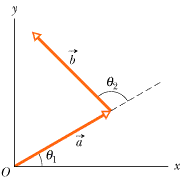
\includegraphics[scale=1]{hw3_problem5}
			\caption{Plot of $y$ versus $x$}
			\label{fig:hw3_problem5}
		\end{center}
	\end{figure}

	\subsection{Question (a)}
		Find the $x$ component of their vector sum $\vec{r}$.

		\textbf{R:} \newline
		\begin{align}
			r_{x} = \ &(a \ \cos{\theta_{a}}) + (b \ \cos{\theta_{b}})& \notag \\
			a = \ &b = 42 \ ft& \notag \\
			\theta_{a} = \ &\theta_{1} = 37^{o}& \notag \\
			\theta_{b} = \ &\theta_{a} + \theta_{2} = 37^{o} + 102^{o} = 139^{o}& \notag \\
			r_{x} = \ &\left[ (42 \ ft) \cos{37^{o}} \right] + \left[ (42 \ ft) \cos{139^{o}} \right]& \notag \\
			= \ &\left[ (42 \ ft) \times (0.799) \right] + \left[ (42 \ ft) \times (- 0.755) \right]& \notag \\
			= \ &(33.558 \ ft) + (-31.710 \ ft)& \notag \\
			= \ &1.848 \ ft&
		\end{align}

	\subsection{Question (b)}
		Find the $y$ component of their vector sum $\vec{r}$.

		\textbf{R:} \newline
		\begin{align}
			r_{y} = \ &(a \ \sin{\theta_{a}}) + (b \ \sin{\theta_{b}})& \notag \\
			r_{y} = \ &\left[ (42 \ ft) \sin{37^{o}} \right] + \left[ (42 \ ft) \sin{139^{o}} \right]& \notag \\
			= \ &\left[ (42 \ ft) \times (0.602) \right] + \left[ (42 \ ft) \times (0.656) \right]& \notag \\
			= \ &(25.284 \ ft) + (27.552 \ ft)& \notag \\
			= \ &52.836 \ ft&
		\end{align}

	\subsection{Question (c)}
		Find the magnitude of $\vec{r}$.

		\textbf{R:} \newline
		\begin{align}
			r = \ &\left| \vec{r} \right| = \sqrt{(1.848 \ ft)^{2} + (52.836 \ ft)^{2}}& \notag \\
			r = \ &\sqrt{(3.415 \ ft^{2}) + (2791.643 \ ft^{2})}& \notag \\
			= \ &\sqrt{2795.058 \ ft^{2}}& \notag \\
			= \ &52.868 \ ft&
		\end{align}

	\subsection{Question (d)}
		Find the angle $\vec{r}$ makes with the positive $x$ axis.

		\textbf{R:} \newline
		\begin{align}
			\theta_{r} = \ &\tan^{-1} \left( \frac{52.836 \ ft}{1.848 \ ft} \right)& \notag \\
			= \ &\tan^{-1} \left( 28.591 \right)& \notag \\
			= \ &88.000^{o}&
		\end{align}
